\section{Rechnerarchitektur}
\subsection{Von-Neumann-Rechner}
Kennzeichen:
\begin{itemize}\itemsep0em
	\item Der Rechner ist universell oder Turing mächtig	
	\item Programm und Daten liegen im gleichen beschreibbaren Speicher auf den beliebig zugegriffen werden kann (RAM -- Random Access Memory). Zwischen Programm und Programmdaten wird nicht unterschieden. Hier ist auch das grösste Risiko. Programm oder Daten können beabsichtigt oder unbeabsichtigt beschädigt werden
	\item Programm und Daten sind binär codiert
	\item Steuerung erfolgt über Befehle in einem Programm
	\item Ohne korrektes Programm ist der Rechner nutzlos
	\item Programm = Sequenz von Anweisungen/Entscheidungen
	\item Der Befehlszähler (spez. Speicher) kennt Adresse des nächsten Befehls
	\item Bedingte Befehle erlauben Entscheidungen über den Fortgang des Programms
\end{itemize}

\subsubsection{Komponenten}
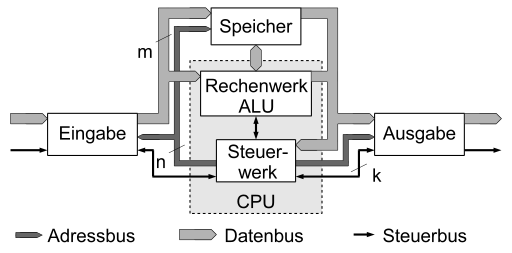
\includegraphics[width=\linewidth]{von_Neumann-_Architektur_de.png}
\begin{description}\itemsep0em
	\item [Steuerwerk] (Leitwerk/\textit{Control Unit}) enthält Befehlsregister, Befehlsdecoder und den Befehlszähler:
	\begin{itemize}
		\item Interpretiert Programmcode
		\item Erstellt Verbindungen zwischen Speicher und Rechenwerk
		\item Steuert die Reihenfolge der Programmbefehle
	\end{itemize}

	\item [Rechenwerk] (Arithmetisch-Logische-Einheit, \textit{Arithmetic Logic Unit (ALU)}) stellt logische und mathematische Operationen (NICHT, ODER, \dots, Addition, Multiplikation, \dots) zur Verfügung

	Steuer- und Rechenwerk zusammen bilden heutzutage zusammen (mit weiteren Komponenten) die \textit{Central Processing Unit (CPU)} (aka. Hauptprozessor)

	\item [Speicher(werk)] (\textit{Memory}) Speichert alle Daten (alles im selben Speicher). Der Speicher ist in fortlaufend durchnummerierte gleich grosse Zellen unterteilt. Die Nummer entspricht der Adresse der Speicherzelle
	\item [Eingabewerk] Steuert die Eingabe aller Daten des Rechners 
	\item [Ausgabewerk] Steuert die Ausgabe aller Daten des Rechners

	Ein- und Ausgabewerk zusammen sind letztendlich dedizierte Speicher. Sie sind heutzutage in der \textit{Input/Output-Unit (I/O-Unit)} zusammengefasst
\end{description}

Die einzelnen Werke sind über Bus-Systeme (Daten-, Adress- und Steuerbus) miteinander verknüpft.

\subsubsection{Register}
Register (Teil des Steuer- und Rechenwerks) sind sehr schnelle, sehr kleine Speicher für die Zwischenspeicherung von Daten. Steuer- und Rechenwerk arbeiten i.\,d.\,R. mit Werten dieser Register

\begin{itemize}\itemsep0em
	\item Befehlsregister (im Steuerwerk)
	\item Befehlszähler (im Steuerwerk)
	\item Zustandsregister (im Steuerwerk)
	\item Interrupt-Register (im Steuerwerk)
	\item Akkumulator (im Rechenwerk)
	\item Statusregister (im Rechenwerk)
	\item Hilfs- und Arbeitsregister (\textit{General Purpuse Register}, Steuer- und Rechenwerk)
\end{itemize}

Die Grösse der Register (i.\,d.\,R. $n \cdot 8$) charakterisiert einen Rechner:
\begin{itemize}\itemsep0em
	\item Akkumulator/Arbeitsregister definiert Grösse der in einem Zyklus bearbeitbaren Zahlen
	(Bei 32 Bit $\rightarrow 2^{32}$ mögliche Zahlen)
	\item Befehlszähler definiert die Grösse des direkt ansprechbaren Speichers
	\item Befehlsregister definiert die Anzahl möglicher Befehle
\end{itemize}
Für Register gilt: je grösser, desto teuerer. Üblich sind 8, 16, 32 und 64 Bit Register

Ein Register besteht aus $n$ Flip-Flops, die einzeln angesprochen werden können

\subsubsection{Programmablauf}
\begin{enumerate}\itemsep0em
	\item Aktuelles Befehlswort aus der Speicherzelle, auf die der Befehlszähler zeigt lesen und and das Steuerwerk übertragen
	\item Befehlswort dekodieren und entsprechende Signale auf die Steuerleitungen schalten
	\item Operanden aus dem Speicherwerk lesen und in die Register des Rechenwerks übertragen
	\item Operation ausführen und Ergebnis in ein Register oder den Speicher schreiben
	\item Befehlszähler um eins erhöhen (oder aufgrund eines Sprungbefehls auf einen anderen Wert setzen)
\end{enumerate}

\subsubsection{Von-Neumann-Flaschenhals}
Die Trennung von Recheneinheit und Speicher führt dazu, dasss Daten sehr häufig übertragen werden müssen. Somit wird der Zuständige Datenbus zum Flaschenhals (Von-Neumann-Flaschenhals).
Auf dem Datenbus werden sowohl Programmcode als auch Daten übertragen und das ganze geschieht sequentiell.

Lösungsansätze:
\begin{itemize}\itemsep0em
	\item Schneller Zwischenspeicher zwischen CPU und Speicher (Cache)
	\item Getrennte Busse und Zwischenspeicher für Programmcode und Daten
	\item Vorhersagen von bedingten Programmverzweigungen (\textit{branch prediction})
	\item Parallele Strukturen
\end{itemize}

\subsection{Harvard-Architektur}
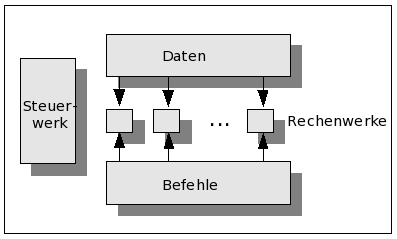
\includegraphics[width=\linewidth]{Harvard-architektur.png}
\begin{itemize}\itemsep0em
	\item Trennt Programm- und Datenspeicher (inkl. Zwischenspeicher)
	\item Nutzt getrennte Datenbusse
	\item kann mehrere Rechenwerke parallel nutzen
\end{itemize}

 \begin{tabular}{@{}p{\linewidth/2}%
				@{}p{\linewidth/2}}
	\multicolumn{1}{c}{\underline{Linksverschiebung}} & \multicolumn{1}{c}{\underline{Rechtsverschiebung}}\\
	Programm und Daten werden gleichzeitig geladen & Nichtdeterministisches Verhalten aufgrund unterschiedlicher Laufzeiten \\
	Programmcode kann nicht überschrieben werden & Nicht genutzer Speicherplatz der einen Art kann nicht für die andere genutzt werden \\
	Befehlswortbreite und Datenwortbreite können unterschiedlich sein & \\

\end{tabular}

\subsubsection{Super-Harvard-Architektur}
Auf gemeinsamen Speicher wird über verschiedene Datenbusse parallel zugegriffen
